\chapter{Heating Effect of Electric Current}

\section{Aim}
To investigate the factors affecting the heat produced by an electric current in a resistor

\section{Background Information}
Electric iron, kettles and heaters produce heat for ironing clothes and raising the temperature of liquids respectively. The heat produced is from current flowing in the metal coils which act like resistors. What factors determine the quantity of heat generated in a resistor due to current flowing through it?

\section{Materials}
3 dry cells (1.5 V size D), resistance wire of length 25 cm, Rheostat, switch, ammeter, voltmeter, calorimeter, thermometer, stirrer, ruler, stopwatch, water and connecting wires.

\section{Procedure}
Case (i)
\begin{enumerate}
\item Put water in a lagged calorimeter until it is about $^2/_3$ full.
\item Connect the circuit consisting of a battery (E), Rheostat (Rh), switch (K), ammeter (A), voltmeter (V) and resistance wire of length $L = 25$ cm (coiled) and a calorimeter (see figure).
\item Place the thermometer and stirrer into the calorimeter.
\item Record initial temperature $\theta_1$ of the water in the colorimeter by using a thermometer.
\item Close the switch K and adjust the rheostat to give suitable values of current $I$ and voltage $V$.
\item Leave the circuit on for 30 minutes and record final temperature $\theta_f$. 
\item Adjust the rheostat to obtain five different values of $I$ and $V$ and record the temperature after each 30 minutes.
\item Record the values of $I$, $V$ and $\Delta \theta$ in a tabular form.
\end{enumerate}
\noindent
Case (ii)
\begin{enumerate}
\item Use the same experimental setup as in case (i).
\item Keep the current $I$, potential difference $V$, and all resistances constant.
\item Record the values of change in temperature $\Delta \theta$ with the corresponding time $t$, at intervals of 15 minutes, in tabular form.
\end{enumerate}
\noindent
Case (iii)
\begin{enumerate}
\item Use the same experimental setup as before.
\item Vary the length, $L$ of the resistance wire by decreasing the length by intervals of 5 cm four times.
\item For each length $L$, allow the current to flow for 30 minutes.
\item Record the length of the resistance wire and the corresponding changes in temperature $\Delta \theta$ in a table.
\end{enumerate}

\begin{figure}[h!]
\centering
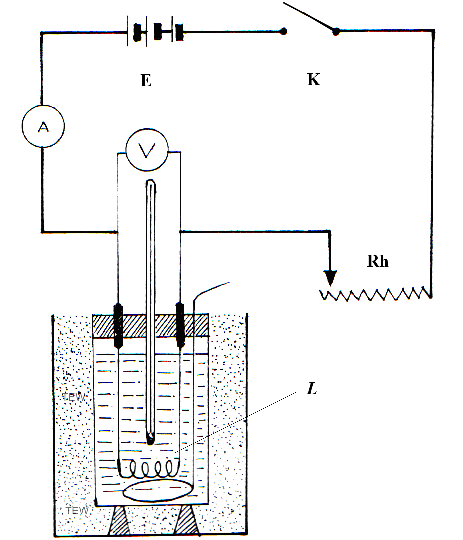
\includegraphics[width=6cm]{./img/heating-effect-current-1.png}
\caption{Heating Effect of Electric Current practical setup}
\label{fig:heating-effect-current-1}
\end{figure}

\section{Safety Measure}
Do not switch on the current until heating coil is in the water.

\section{Analysis and Interpretation}
\begin{enumerate}
\item Plot the graph of:
\begin{itemize}
\item[(i)] Temperature change $\Delta \theta$ against the square of current $I^2$ and explain the nature of the graph.
\item[(ii)]	Temperature change $\Delta \theta$ against time $t$ and explain the nature of the graph.
\item[(iii)] Temperature change $\Delta \theta$ against length $L$.
\end{itemize}
\end{enumerate}

\section{Conclusion}
What are the various factors affecting the heat produced by current flowing through a resistor and what are their relationships with the quantity of heat produced?

\section{Questions for Discussion}
\begin{enumerate}
\item Why should you not close the switch before placing the heater coil in the water?
\item Why is it better to use nichrome wire for the heater rather than copper wire?
\item What is the purpose of performing the experiment with specific factors kept constant and others not?
\item What are the sources of error and suggest ways to minimize them?
\item Construct an equation using the results of these experiments to relate the total heat generated to the resistance, current and the time of current flow. Note: the proportionality constant is equal to 1. 
\item Why do heating coils have a large number of turns?
\end{enumerate}

\section{Reflection and Self Assessment}
\begin{enumerate}
\item What were the most and least interesting parts of this experiment to you? Explain.
\item How can you use the results of this experiment in your daily life? 
\end{enumerate}